\chapter{Teorema de Lax-Milgran}

Para dejar el puente libre, primero necesitamos ver nuestro funcional $L$ desde otro punto de vista. Para ello, vamos a ver una serie de definiciones y propiedades abstractas sobre los \textit{funcionales cuadráticos}, lo que nos va a permitir enunciar el teorema de Lax-Milgran, que nos dará la existencia de solución en esta última versión del modelo.

\begin{definition}\label{formabilineal}
Dados un cuerpo $K$ y un $K-$espacio vectorial $V$, una forma bilineal es una aplicación $\funcion{f}{V\times V}{K}$ que verifica:
\begin{enumerate}[(a)]
\item $f(u_1+u_2,v)=f(u_1,v)+f(u_2,v)$
\item $f(u, v_1+v_2)=f(u,v_1)+f(u,v_2)$
\item $f(au,v)=af(u,v)$
\item $f(u,av)=af(u,v)$
\end{enumerate}
para cualquier $a\in K$ y $u,v,u_1,u_2,v_1,v_2\in V$.

Una propiedad que necesitaremos es:
\[
f\left(\sum_ia_iu_i,\sum_jb_jv_h\right)=\sum_i\sum_ja_ib_jf(u_i,v_j)
\]

\end{definition}

\begin{definition}
Una forma bilineal $\funcion{f}{V\times V}{K}$ se dice simétrice si verifica:
\[
f(u,v)=f(v,u) \espacio \forall u,v\in V
\]
\end{definition}

\begin{definition}
Sea $H$ un espacio de Hilbert arbitrario, $\funcion{A}{H\times H}{\R}$ una forma bilineal, continua y simétrica y $\funcion{R}{H}{\R}$ una aplicación lineal y continua. Llamamos funcional cuadrático a la aplicación $\funcion{L}{H}{\R}$ dada por
\[
L(y)=\frac{1}{2}A(y,y)-R(y) \espacio\forall y\in H
\]
\end{definition}

\begin{definition}
Sea $\funcion{L}{H}{\R}$ una forma cuadrática. Diremos que es coerciva si existe una constante $\alpha\in\R^+$ tal que:
\[
A(u,u)\geq \alpha\norm{u}^2 \espacio \forall u\in H
\]
\end{definition}

\begin{prop}
Sea un espacio de Hilbert $H$ y $\funcion{L}{H}{\R}$ una forma cuadrátrica en ese espacio.
Entonces, la aplicación $\funcion{\norm{\cdot}_H}{H}{\R^+_0}$ definida por 
\[
\norm{u}_H=\sqrt{A(u,u)} \espacio \forall u\in H
\]
donde $\funcion{A}{H\times H}{\R}$ es la forma bilineal asociada a $L$, es una norma, y es equivalente a la norma natural de $H$.
\end{prop}
\begin{proof}
El hecho de que $\norm{\cdot}_H$ es una norma es sencillo de comprobar ya que $A$ define un producto escalar en $H$.

Sea $\funcion{\norm{\cdot}}{H}{\R}$ la norma de $H$. Necesitamos encontrar dos constante $c_1,c_2\in\R^+$ tal que 
\[
c_1\norm{u}\leq \norm{u}_H \leq c_2\norm{u}
\]
La constante $c_2$ la obtenemos por continuidad de la norma $\norm{\cdot}_H$ y la constante $c_1$ de la coercividad de $L$.

\end{proof}
A partir de ahora consideramos $\norm{\cdot}_H$ como nuestra norma por defecto en $H$.
\begin{prop}
Todo funcional cuadrático está acotado inferiormente.
\end{prop}
\begin{proof}
Sea $\funcion{L}{H}{\R}$ un funcional cuadrático, donde $\funcion{A}{H\times H}{\R}$ es su forma bilineal, continua y simétrica y $\funcion{R}{H}{\R}$ es su aplicación lineal y continua.
Vamos a ver que podemos acotar inferiormente la expresión de $L(y)$, con $y\in H$, por una función parabólica hacia arriba.

Como $R$ es continua, entonces $\norm{R(y)}\leq \norm{R}\norm{y} \Rightarrow -\norm{R(y)} \geq -\norm{R}\norm{y}$. Además, como $L$ es coerciva, existe cierta constante $C\in\R^+$ tal que $A(y,y)\geq C\norm{y}^2$. Combinando esas dos acotaciones, obtenemos:
\[
L(y)=\frac{1}{2}A(y,y)-R(y)\geq \frac{1}{2}C\norm{y}^2-\norm{R}\norm{y}
\]
Para ver con más claridad la parábola, hacemos el cambio $s=\norm{y}$, obteniendo una nueva función $P$ dependiente de las dos constantes $C$ y $\norm{R}$: $P(s)=\frac{1}{2}s^2-s\norm{R}$. Derivando e igualando a 0, obtenemos fácilmente que el mínimo de la parábola $P$ se alcanza en $s=\frac{\norm{R}}{C}$. Luego:
\[
L(y)\geq \frac{\norm{R}}{C} \espacio \forall y\in H 
\]

\end{proof}

\begin{theorem}[Lax-Milgran]
\label{laxmilgran}
Sea $\funcion{L}{H}{\R}$ un funcional cuadrático. Si $L$ es coercivo, entonces tiene mínimo absoluto en $H$.
\end{theorem}

\begin{prop}[condición de punto crítico]
\label{puntocritico}
Sea $\funcion{L}{H}{\R}$ un funcional cuadrático coercivo, $y\in H$, $\phi\in\soportecompacto$. Entonces existe $y\in H$ verificando:
\[
A(\phi,y)-R(\phi)=0 \espacio \forall\phi\in\soportecompacto
\]

Además, el punto $y$ es el mínimo de $L$.
\end{prop}
\begin{proof}
Calculemos primero la expresión explícita de $g(s)$:
\[
g(s)=L(y+s\phi)=\frac{1}{2}A(y+s\phi,y+s\phi)-R(y+s\phi)
\]
Desarrollamos el primer término (usando la última propiedad en la definición \ref{formabilineal}):
\[
A(y+s\phi,y+s\phi)=A(y,y)+sA(y,\phi)+sA(\phi,y)+s^2A(\phi,\phi)=s^2A(\phi,\phi)+2sA(\phi,\phi)+A(y,y)
\]
Para el segundo término, usamos que $R$ es lineal:
\[
R(y+s\phi)=R(y)+sR(\phi)
\]
Quedándo:
\[
g(s)=\frac{1}{2}\left(s^2A(\phi,y)+2sA(\phi,\phi)+A(y,y)\right)-R(y)-sR(\phi)
\]
Derivando respecto de $s$:
\[
g(s)=sA(\phi,\phi)+A(\phi,y)-R(\phi) \Rightarrow g'(0)=A(\phi,y)-R(\phi)
\]
Luego nuestra condición de punto crítico es:
\[
A(\phi,y)-R(\phi)=0 \espacio \forall\phi\in\soportecompacto
\]

Para le existencia, simplemente tenemos que definir un producto escalar y usar el teorema de Riesz, como en los ejemplos anteriores. Sea $<<u,v>>=A(u,v)$ un producto escalar en $H$, por el teorema \ref{riesz-frechet}, existe $y\in H$ verificando:
\[
<<y,\phi>>=R(\phi) \espacio \forall \phi\in\soportecompacto
\]

Para ver que es mínimo, tomamos $\funcion{g}{\R}{\R}$ definida por $g(s)=L(y+s(z-y))$. Notemos que $y+s(z-y)$ es la recta que una a $z$ con $y$. Tenemos que ver
\[
L(z)>L(y) \espacio \forall z\in H
\]
Que si nos fijamos, es equivalente a ver que
\[
g(1)>g(0)
\]
Que ya lo tenemos porque $s=0$ era el punto mínimo de la parábola.
\end{proof}

Una vez planteada toda la teoría necesaria, podemos volver a nuestro modelo del puente. Recordemos que nuestro funcional  $\funcion{L}{\sobolev{1}}{\R}$ venía dado por la expresión:
\[
L(y)=\frac{1}{2}\integral{a}{b}{y'(x)^2dx}+\frac{1}{2}\integral{a}{b}{K(x)y(x)^2dx}+\integral{a}{b}{q(x)y(x)dx}
\]
donde $q,K\in\lebesgue{\infty}$ y $K(x)\geq k_0 >0\casipordoquier$. La última condición la imponemos porque al dejar los extramos sueltos (lo hemos hecho al considerar como dominio de $L$ el espacio $\sobolev{1}$ en lugar de $\sobolevcero{1}$) necesitemos que el puente siga enganchado por las cuerdas.

Para poder usar la teoría desarrollada anteriormente, necesitamos ver que nuestro funcional es cuadrático. Definimos nuestra forma bilineal, continua y simétrica, y nuestra aplicación lineal y continua:
\[
A(u,v)=\integral{a}{b}{u'(x)v'(x)dx}+\integral{a}{b}{K(x)u(x)v(x)dx}, \; \espacio R(u)=-\integral{a}{b}{q(x)u(x)dx} \;\;\forall u,v\in\sobolev{1}
\]
Pero también necesitamos que $L$ sea coerciva. Usando la hipótesis sobre $K(x)$ es fácil de ver:
\[
A(u,u)=\integral{a}{b}{u'(x)^2dx}+\integral{a}{b}{K(x)u(x)^2dx}\geq\normasobolev{1}{u}^2+k_0\normasobolev{1}{u}^2\geq(1+k_0)\normasobolev{1}{u}^2
\]
Por lo tanto, sabemos que existe mínimo en $\sobolev{1}$. Además de saber que existe, queremos saber algo más sobre su expresión. Como hemos visto antes, los puntos críticos están caracterizados por la expresión:
\[
y\in\sobolev{1} \text{ punto critico } \Leftrightarrow A(y,\phi)=R(\phi) \espacio \forall \phi\in\sobolev{1}
\]
es decir,
\[
\integral{a}{b}{y'(x)\phi'(x)dx}+\integral{a}{b}{K(x)y(x)\phi(x)dx}=-\integral{a}{b}{q(x)\phi(x)dx} \espacio  \forall\phi\in\sobolev{1}
\]
Si en lugar de considerar $\phi$ en $\sobolev{1}$, la consideramos en $\soportecompacto$. Vemos que llamando $z=y'$ y agrupando los términos que tienen $\phi$, llegamos a:
\[
\integral{a}{b}{z(x)\phi'(x)dx}=-\integral{a}{b}{(K(x)y(x)+q(x))\phi(x)dx} \espacio  \forall\phi\in\sobolev{1}
\]

lo que significa que la derivada débil de $z$ es justamente $ky+q$. En particular z está en $\sobolev{1}$, porque todas las funciones que aparecen están en $\lebesgue{2}$. Luego debemos resolver la siguiente ecuación diferencial de orden 2 en $y$:
\[
y''(x)=K(x)y(x)+q(x) \espacio \forall x \in[a,b]
\]
Si imaginamos que $K$ y $q$ son continuas, esa ecuación tendría un gran número de soluciones. De hecho, el conjunto de soluciones sería un espacio biparamétrico (porque la solución depende de las condiciones iniciales sobre $y$ e $y'$). Tenemos que intentar limitarlas de alguna forma.

\begin{prop}
Sea $y\in\sobolev{1}$ (el representante continuo) y $\phi\in\mathcal{D}(\R)$, entonces $y\phi\in\sobolev{1}$.
\end{prop}
\begin{proof}
Para ver que $y\phi\in\sobolev{1}$, necesitamos encontrar su derivada débil. ¿Cuál es nuestro candidato a derivada débil? La derivada clásica, es decir, $z=y'\phi+y\phi'$. Para comprobarlo, tenemos que ver que para toda $\psi\in\soportecompacto$ se tiene:
\[
\integral{a}{b}{(y'(x)\phi(x)+y(x)\phi'(x))\psi(x)dx}+\integral{a}{b}{y(x)\phi(x)\psi'(x)dx}=0
\]
Reordenando los términos que tienen $y$ e $y'$, obtenemos:
\[
\integral{a}{b}{(\phi(x)\psi'(x)+\phi'(x)\psi(x))y(x)dx}+\integral{a}{b}{\phi(x)\psi(x)y'(x)dx}=0
\]
Luego
\[
\integral{a}{b}{y'(x)\phi(x)}+\integral{a}{b}{y(x)\phi'(x)}=y(x)\phi(x)\Big|^b_a
\] 
\textbf{DEMOSTRACION DUDOSA}
\end{proof}

\section{La delta de Dirac y el espacio $H^{-1}$}
\subsection{Caso particular}
Ahora vamos a ver otro caso del modelo, donde colgamos una masa $m$ en un punto $\alpha\in(a,b)$ del puente. La energía de este objeto es $my(\alpha)$, luego la expresión de nuestro funcional $\funcion{L}{\sobolevcero{1}}{\R}$ es:
\[
L(y)=\frac{1}{2}\integral{a}{b}{y'(x)^2dx}+\frac{1}{2}\integral{a}{b}{q(x)y(x)^2dx}+my(\alpha)
\]
donde $y\in\sobolevcero{1}$, $q(x)\geq 0$ y  $q\in\lebesgue{\infty}$. La intuición nos dice que al colgar la masa $m$, se formará un pico en la cuerda, como muestra el siguiente dibujo:

\begin{center}
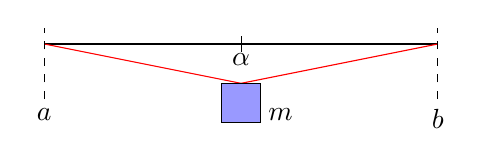
\begin{tikzpicture}
\draw (0,0) -- (5,0);
% parabola
\draw[scale=1,domain=0:2.5,smooth,variable=\x,red] plot ({\x}, {-0.2*\x});
\draw[scale=1,domain=2.5:5,smooth,variable=\x,red] plot ({\x}, {0.2*(\x-5)});

% etiquetas
\draw[dashed] (0,-0.7) -- (0,.2);
\draw (0,-0.7) node[anchor=north] {$a$};
\draw[dashed] (5,-.7) -- (5,.2);
\draw (5,-0.7) node[anchor=north] {$b$};
\draw (2.5,-0.1) -- (2.5,.1);
\draw (2.5,0) node[anchor=north] {$\alpha$};
\draw (3,-0.7) node[anchor=north] {$m$};

% masa
\fill[blue!40!white, draw=black] (2.25,-1) rectangle (2.75,-0.5);
\end{tikzpicture}
\end{center}
La forma bilineal $A$ es la misma que en el anterior modelo:
\[
A(y,y)=\frac{1}{2}\integral{a}{b}{y'(x)^2dx}+\frac{1}{2}\integral{a}{b}{q(x)y(x)^2dx}
\]
y como estamos en $\sobolevcero{1}$, $\integral{a}{b}{y'(x)^2dx}$ es una norma, luego $A$ es coercivo ya que restando el último término (que es positivo) obtenemos:
\[
A(y,y)\geq \frac{1}{2}\integral{a}{b}{y'(x)^2dx} = \frac{1}{2}\norm{u}^2
\] 
La aplicación lineal y continua $\funcion{R}{\sobolevcero{1}}{\R}$, viene dada por $R(y)=-my(\alpha)$, que tiene sentido al elegir el represante continuo porque $\sobolev{1}\subset \mathcal{C}(a,b)$. Por el teorema de Lax-Milgran (\ref{laxmilgran}) y la proposicion \ref{puntocritico}, existe $y\in\sobolevcero{1}$ de forma que
\[
A(y,\phi)=R(\phi) \espacio \forall \phi\in\sobolevcero{1}
\]
Lo que vamos a hacer ahora es calcular o ver qué condiciones verifica la función $y$. Usando la condición de punto crítico:
\begin{equation}
\label{formulageneral}
\integral{a}{b}{y'(x)\phi'(x)dx}+\integral{a}{b}{q(x)y(x)\phi(x)dx}=-m\phi(\alpha)
\end{equation}
Ahora hacemos una distinción de casos con $\phi$ perteneciendo a diferentes clases de Swartz:
\begin{itemize}[-]
\item si $\phi\in\mathcal{D}(a,\alpha)$:
\[
\integral{a}{b}{y'(x)\phi'(x)dx}+\integral{a}{b}{q(x)y(x)\phi(x)dx}=-m\phi(\alpha)=0
\]
ya que $\alpha\notin(a,\alpha) \Rightarrow \phi(\alpha)=0$. Si denotamos $z=y'$, entonces $z\in\sobolev[a,\alpha]{1}\subset\mathcal{C}[a,\alpha]$ (porque la expresión anterior coincide con la definición de derivada débil para $z$).
\item si $\phi\in\mathcal{D}(\alpha,b)$, de igual forma conseguimos que $z\in\sobolevcero[\alpha,b]{1}\subset\mathcal{C}[\alpha,b]$. 
\end{itemize}
Fijaros que ese razonamiento no implica que $z\in\mathcal{C}[a,b]$, ya que el representante continuo usado en $[a,\alpha]$ y $[\alpha,b]$ son distintos. Lo que si implica es que $z\in\mathcal{C}\left([a,\alpha)\cup(\alpha,b]\right)$ y existen los límites laterales de $\alpha$:
\[
z(\alpha^-)=\limite{x}{\alpha^-}{z(x)} \espacio z(\alpha^+)=\limite{x}{\alpha^+}{z(x)}
\]
Además sabesmos que $z'=qy \;\; a.e \; x \in(a,\alpha)\cup(\alpha,b)$. Si volvemos a la fórmula general \eqref{formulageneral}:
\begin{equation}
\label{formulageneral2}
\integral{a}{b}{z(x)\phi'(x)dx}+\integral{a}{b}{q(x)y(x)\phi(x)dx}=-m\phi(\alpha) \espacio \forall\phi\in\sobolevcero{1}
\end{equation}
Ahora queremos desarrollar esa expresión. Tomamos $\phi\in\soportecompacto$, como $z$ no es continua en $\alpha$, la integral del primer término hay que escribirla en dos partes:
\[
\integral{a}{b}{z(x)\phi'(x)dx}=\integral{a}{\alpha}{z(x)\phi'(x)dx}+\integral{\alpha}{b}{z(x)\phi'(x)dx}
\]
Aplicamos derivación por partes a cada término:
\[
\integral{a}{\alpha}{z(x)\phi'(x)dx}=z(x)\phi(x)\Big|_a^\alpha-\integral{a}{\alpha}{z'(x)\phi(x)dx}=z(\alpha^-)\phi(\alpha)-\integral{a}{\alpha}{z'(x)\phi(x)dx}
\]
\[
\integral{\alpha}{b}{z(x)\phi'(x)dx}=z(x)\phi(x)\Big|_\alpha^b-\integral{\alpha}{b}{z'(x)\phi(x)dx}=-z(\alpha^+)\phi(\alpha)-\integral{\alpha}{b}{z'(x)\phi(x)dx}
\]
Combinando los resultados y sustituyendo en \eqref{formulageneral2}:
\[
z(\alpha^-)\phi(\alpha)-z(\alpha^+)\phi(\alpha)-\integral{a}{b}{z'(x)\phi(x)dx}=-\integral{a}{b}{z'(x)\phi(x)dx}-m\phi(\alpha)
\]
Cancelando ámbos términos:
\[
\left(z(\alpha^-)-z(\alpha^+)\right)\phi(\alpha)=-m\phi(\alpha)
\]
Como la función de Swartz esocgido es arbitraria, podemos suponer quevale 1 en $\alpha$. Usando eso y que $z=y'$:
\[
y'(\alpha^-)-y'(\alpha^+)=-m \Rightarrow y'(\alpha^+)-y'(\alpha^-)=m  
\]
Es decir, el cambio de pendiente que se da entre $\alpha^-$ y $\alpha^+$ es igual a $m$, el peso de la masa.

\duda{entre este apartado y el siguiente hay varias cosas que se repiten, como el planteamiento del funcional, el problema de sutrm-liouville, etc, me gustaría saber que se debería quedar y que debería borrar}

\subsection{Caso abstracto: problema de Sturm-Liouville}
Vamos a generalizar el caso anterior para obtener una ecuación diferencial con varias condiciones. Sea $\funcion{L}{\sobolev{1}}{\R}$ el funcional dado por:
\[
L(y)=\frac{1}{2}\integral{a}{b}{p(x)y'(x)^2dx}+\frac{1}{2}\integral{a}{b}{q(x)y(x)dx}-R(y)
\]
donde $p,q\in\lebesgue{\infty}$ cumpliendo $0<p_0\leq p(x)\leq p_1$, $0<q_0\leq q(x)\leq q_1$. 

La teoría de Lax-Milgran nos dice que:
\[
A(y,\phi)=R(\phi) \Rightarrow \integral{a}{b}{p(x)y'(x)\phi'(x)dx}+\integral{a}{b}{q(x)y(x)\phi(x)dx}=R(\phi)
\]
Y denotando $z=py'$ se verifica $z'=qy-R(\phi)$.

\begin{definition}
Sean $p,q\in\lebesgue{\infty}$ cumpliendo $0<p_0\leq p(x)\leq p_1$, $0<q_0\leq q(x)\leq q_1 \;\; \casipordoquier$. La ecuación de Sturm-Liouville viene dada por la expresión:
\[
(p(x)y'(x))'-q(x)y(x)=R(\phi)
\]
\begin{itemize}
\item Si $y\in\sobolevcero{1}$, consideramos $R\in(\sobolevcero{1})^*$.
\item Si $y\in\sobolev{1}$, consideramos $R\in(\sobolev{1})^*$.
\end{itemize}
\end{definition}
\begin{definition}
Una solución débil de la ecuación de Sturm-Lioville es una función $y$ verificando la expresión anterior.
\begin{itemize}
\item Si $y\in\sobolevcero{1}$, entonces $y(a)=y(b)=0$ (caso Dirichlet).
\item Si $y\in\sobolev{1}$, entonces $y'(a)=y'(b)=0$ (caso Neumann).
\end{itemize}
\end{definition}
\begin{remark}
Si consideramos $R\in(\sobolev{1})^*$, la condición $y'(a)=y'(b)=0$ nos aparece de forma natural al minimizar (visto anteriormente).
\end{remark} 

A partir de ahora nos vamos a centrar en el caso $y\in\sobolev{1}$, $R\in(\sobolev{1})^*$.

\textbf{que vamos a hacer a continuacion?}

\begin{remark}
Recordemos una propiedad del Análisis funcional respecto a duales: (\textbf{DUDOSA})
\begin{center}
\begin{tikzpicture}[node distance=2.5cm, auto]
\node (A) {$\sobolev{1}$};
\node (B) [right of=A] {$\sobolev{1}$};
\node (C) [below of=A] {$(\sobolev{1})^*$};
\node (D) [below of=B] {$(\sobolev{0})^*$};
\draw[->](A) to node {$i$}(B);
\draw[->, dashed](B) to node [] {}(D);
\draw[->, dashed](A) to node [] {}(C);
\draw[->](D) to node [above] {$i^*$}(C);
\end{tikzpicture}
\end{center}
donde $i^*$ es la aplicación traspuesta de $i$. Veámoslo con un ejemplo concreto, supongamos que tenemos $n<m$:
\begin{center}
\begin{tikzpicture}[node distance=2cm, auto]
\node (A) {$\R^n$};
\node (B) [right of=A] {$\R^m$};
\node (C) [below of=A] {$\R^n$};
\node (D) [below of=B] {$\R^m$};
\draw[->](A) to node {$i$}(B);
\draw[->, dashed](B) to node [] {}(D);
\draw[->, dashed](A) to node [] {}(C);
\draw[->](D) to node [above] {$i^*$}(C);
\end{tikzpicture}
\end{center}
donde $i\in\mathcal{M}_{n\times m}$ y $i^*\in\mathcal{M}_{m\times n}$. Lo esperable es que si $i$ es inyectiva, es decir, el rango de $i$ es $n$, entonces la otra matriz también tiene rango $n$, pero eso quiere decir que es sobreyectiva. Es decir, esta dualidad nos pasa aplicaciones inyectivas a aplicaciones sobreyectivas. A nosotros nos interesa ver la inclusión de los espacios "relativamente bien", puesto que el al fin y al cabo el Teorema de Riesz nos dice que todos los espacios de Hilbert son iguales, pero no quiero perder la estructura ni las inclusiones entre ellos.
\end{remark}

\duda{no me queda claro el propósito de esta nota}

Si ahora tomamos $g\in\lebesgue{2}=\sobolev{0}$, podemos definir la función $\funcion{R_g}{\sobolev{1}}{\R}$ por
\[
R_g(y)=\integral{a}{b}{g(x)y(x)dx} 
\]

Aquí dijimos $R_g\in(\sobolev{1})^*=\sobolev{-1}$. Tambíen hablamos de la inclusión
\[
\sobolev{2}\subset\sobolev{1}\subset\sobolev{-1}
\]

\begin{definition}
Dado $\alpha\in(a,b)$, definimos la función $\funcion{\delta_\alpha}{\sobolev{-1}}{\R}$
\[
\delta_\alpha(y)=y(\alpha), \espacio \delta_\alpha\in\sobolev{1}, \;\; \delta_\alpha\notin\sobolev{0}
\]
A $\delta_\alpha$ se le llama $\delta$ de Dirach.
\end{definition}

\duda{no sé que significa lo de abajo}

\[
(py')'-qy=\delta_\alpha
\]
\[
(py')(\alpha^+)-(py')(\alpha^-)=+1
\]

\duda{duda generalizada del caso Dirichlet caso Neumann, según he ententido: antes de esta nota hemos definido el problema de Sturm-Liouville, y ahora consideramos dos casos diferentes (dirichlet y neumann) según donde tomemos la y???}

\subsection{Problema de Sturm-Liouville}
Vamos a escribir formalmente el problema de Sturm-Liouville. Para ello, tomamos el siguiente funcional: 
\[
L(y)=\frac{1}{2}\integral{a}{b}{p(x)y'(x)^2dx}+\frac{1}{2}\integral{a}{b}{q(x)y(x)^2dx}-R(y)
\]
con $p,q\in\lebesgue{\infty}$, $0<p_0\leq p(x)\leq p_1 \; \casipordoquier$. 

Existen dos casos distintos de este problema, dependiendo de donde consideremos la función $y$, es decir, dependiendo de donde queramos minimizar:
\begin{definition}[Caso Dirichlet]
Sea $\funcion{L}{\sobolevcero{1}}{\R}$ y establecemos las siguientes condiciones:
\begin{enumerate}[(a)]
\item $y\in\sobolevcero{1}: \; y(a)=y(b)=0$
\item $0\leq q(x)\leq q_1 \; \casipordoquier$
\item $R\in(\sobolevcero{1})^*$
\end{enumerate}
\end{definition}
\begin{definition}[Caso Neumann]
Sea $\funcion{L}{\sobolev{1}}{\R}$ y establecemos las siguientes condiciones:
\begin{enumerate}[(a)]
\item $y\in\sobolev{1}: \; y'(a)=y'(b)=0$
\item $0<q_0\leq q(x)\leq q_1 \; \casipordoquier$
\item $R\in(\sobolev{1})^*=\sobolev{-1}$
\end{enumerate}
\end{definition}
\begin{remark}
A partir de ahora, cuando pongamos \circled{D} o \circled{N}, haremos referencia a las condiciones del caso Dirichlet o Neumann respectivamente.
\end{remark}
\duda{se ha hablado en varias ocasiones sobre las condiciones que se imponen, pero no me acaban de quedar clara porque imponemos cada una, podría añadir un breve comentario sobre cada una de ellas?}
En cualquiera de los dos casos, el teorema de Lax-Milgran (\ref{laxmilgran}) nos confirma la existencia de solución y nos da la condición de punto crítico (dependiente del caso en el que estemos):
\begin{equation}
\label{criticoliouville}
A(y,\phi)=R(\phi) \Rightarrow \integral{a}{b}{p(x)y'(x)\phi'(x)dx}+\integral{a}{b}{q(x)y(x)\phi(x)dx}=R(\phi)
\end{equation}
\begin{itemize}
\item Para toda $\phi$ en $\sobolevcero{1}$, en el caso Dirichlet.
\item Para toda $\phi$ en $\sobolev{1}$, en el caso Neumann.
\end{itemize}
Formalmente, si llamo $z(x)=p(x)y'(x)$, la expresión \eqref{criticoliouville} me diría que $z'(x)=q(x)y(x)-R$. Fijaros que $R$ no es una función, sino un elemento del dual y que lo único que sabemos es que $y$ está en $\sobolev{1}$, luego no tenemos información sobre $z$. 

Esa ecuación se escribe formalmente como:
\[
(p(x)y'(x))'-q(x)y(x)=R \text{ (Problema de Sturm-Liouville) }
\]
junto con una condición \circled{D} o \circled{N}. 

Si ahora a $R$ la denotamos por $f$, la ecuación quedaría:
\begin{equation}
\label{problemaliouville2}
(p(x)y'(x))'-q(x)y(x)=f(x)
\end{equation}
Fijaros que hemos añadido $(x)$ al lado de $f$, pero realmente $f$ no es una funcion, sino que es un elemento de $(\sobolevcero{1})^*$ (caso \circled{D}) o de $\sobolev{1}$ (caso \circled{N}). Pero recordad que $\lebesgue{2}=\sobolev{0}\hookrightarrow\sobolev{-1}$, ¿cómo hacemos esa inclusión? Con $R_g$, definida anteriormente:
\[
f\mapsto R_f(y)=\integral{a}{b}{f(x)y(x)dx}
\]
\duda{a parte, $R_f(y)\in\R$, cómo va a estar en $\sobolev{1}$ si eso es un espacio de funciones?}
\duda{aqui usamos $R_f$, definido en la clase anterior pero no me queda claro por qué}

\begin{itemize}
\item Si $f\in\sobolev{0} \Rightarrow p(x)y'(x)\in\sobolev{1}$ y tenemos la siguiente ecuación diferencial
\[
(p(x)y'(x))'-q(x)y(x)=f(x)
\]
más la condición \circled{N}, donde esas derivadas sí son débiles.
\item Si $f=\displaystyle\sum_{i=1}^kc_i\delta_{\alpha_i}$ donde $a<\alpha_1,...,\alpha_k<b$ y $c_1,...,c_k\in\R$.

Denotando $z(x)=p(x)y'(x)$, tenemos que $z$ verifica la expresión \eqref{problemaliouville2}:
\begin{equation}
\label{intentandoentenderesto}
\integral{a}{b}{z(x)\phi'(x)dx}+\integral{a}{b}{q(x)y(x)\phi(x)dx}=\sum_{i=0}^kc_i\delta_{\alpha_i}=\sum_{i=0}^kc_i\phi(\alpha_i)
\end{equation}
para toda $\phi$ en $\sobolevcero{1}$ si \circled{D} o en $\sobolev{1}$ si \circled{N}.

Si ahora tomamos $\phi\in\mathcal{D}(a,b)$ de forma que en cada intervalo $(\alpha_{i-1},\alpha_{i+1})$ se cumpla:
\begin{figure}[H]
   \center
  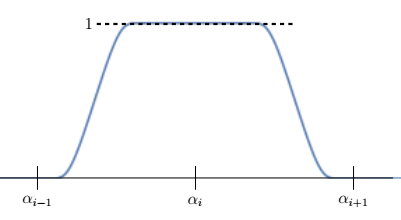
\includegraphics[scale=0.6]{img/flatproof.png}
\end{figure}
y consideramos $z$ como la unión de los representantes continuos en cada intervalo, es decir,
$z\in\mathcal{C}\left([a,\alpha_1)\cup...\cup(\alpha_k,b]\right)$, tenemos que $z'(x)=q(x)y(x) \; \casipordoquier$. Aplicando la expresión \eqref{intentandoentenderesto} a cada intervalo $((\alpha_{i-1},\alpha_{i+1}))$ nos queda:
\begin{equation}
\label{comparando}
\integral{\alpha_{i-1}}{\alpha_{i+1}}{z(x)\phi'(x)dx}+\integral{\alpha_{i-1}}{\alpha_{i+1}}{z'(x)\phi(x)dx}=c_i\phi(\alpha_i)
\end{equation}
Si separamos la integral del primer término en dos, en los intervalos $(\alpha_{i-1},\alpha_{i})$ y $(\alpha_{i},\alpha_{i+1})$ y aplicamos la regla de la cadena:
\[
\integral{\alpha_{i-1}}{\alpha_{i}}{z(x)\phi'(x)dx}=z(x)\phi(x)\Big|_{\alpha_{i-1}}^{\alpha_{i}}-\integral{\alpha_{i-1}}{\alpha_{i}}{z'(x)\phi(x)dx}=z(\alpha_{i}^-)-\integral{\alpha_{i-1}}{\alpha_{i}}{q(x)y(x)\phi(x)dx}
\]
\[
\integral{\alpha_{i}}{\alpha_{i+1}}{z(x)\phi'(x)dx}=z(x)\phi(x)\Big|_{\alpha_{i}}^{\alpha_{i+1}}-\integral{\alpha_{i}}{\alpha_{i+1}}{z'(x)\phi(x)dx}=-z(\alpha_{i}^+)-\integral{\alpha_{i}}{\alpha_{i+1}}{q(x)y(x)\phi(x)dx}
\]
Sumando ahora esos dos resultados y volviendo a combinar las integrales:
\[
\integral{\alpha_{i-1}}{\alpha_{i+1}}{z(x)\phi'(x)dx}=z(\alpha_{i}^-)-z(\alpha_{i}^+)-\integral{\alpha_{i-1}}{\alpha_{i+1}}{q(x)y(x)\phi(x)dx} \Rightarrow
\]
\[
\integral{\alpha_{i-1}}{\alpha_{i+1}}{z(x)\phi'(x)dx}-\integral{\alpha_{i-1}}{\alpha_{i+1}}{q(x)y(x)\phi(x)dx}=z(\alpha_{i}^-)-z(\alpha_{i}^+)
\]
Si nos fijamos, a la izquierda tenemos lo mismo que en la expresión \eqref{comparando}, luego igualando:
\[
z(\alpha_{i}^-)-z(\alpha_{i}^+)=c_i\phi(\alpha_i)=c_i \Rightarrow
\]
\[
z(\alpha_{i}^+)-z(\alpha_{i}^-)=-c_i
\]
\duda{que hemos conseguido con esto?}
\end{itemize}